\subsection{Appearance of Period Adding}

\subsubsection{Horizontal}

\begin{figure}
    \centering
    \subfloat[Regions]{
        \includegraphics[width=.3 \textwidth]{62_MinimalRepr_Adding/2D_Regions_2.8_add_hor/Manual/result.png}
    }
    \subfloat[At point $A$]{
        \includegraphics[width=.3 \textwidth]{62_MinimalRepr_Adding/Cob_2.8_add_hor_A/Manual/result.png}
        \label{fig:minrep.add.app.hor.A}
    }
    \subfloat[At point $B$ \todo{replace figure}]{
        \includegraphics[width=.3 \textwidth]{62_MinimalRepr_Adding/Cob_2.8_add_hor_A/Manual/result.png}
        \label{fig:minrep.add.app.hor.B}
    }
    \caption{Appearance of the horizontal period-adding cascade}
\end{figure}

At point $A$ there is space between the two ``type A'' parameter regions $P_{11}^{4}$ and $P_{10}^{4}$, which overlap at point $B$.
This space opens up more as we change the parameters as described in \Cref{sec:minrep.adding.disapp.typeB}.
Here will be the horizontal period adding region.
\Cref{fig:minrep.add.app.hor.A} shows the cobweb diagram at this point.
The two coexisting cycles $\Cycle{\A^7\B^4\C^6\D^4}$ and $\Cycle{\A^6\B^4\C^7\D^4}$ are asymmetrical like in ``type B'' parameter regions.
But they are different from ``type B'' cycles because they are not of the form $\Cycle{\A^a\B^b\C^{a-1}\D^{b+1}}$ and $\Cycle{\A^{a-1}\B^{b+1}\C^a\D^b}$, but of the form $\Cycle{\A^a\B^b\C^{a-1}\D^b}$ and $\Cycle{\A^{a-1}\B^b\C^a\D^b}$.

If we interpret these cycles in the context of the halved model, this is the first stage of the period-adding cascade.
The two ``type A'' cycles $P_{11}^4$ and $P_{10}^4$ are $\Cycle{\L^7\R^4}$ and $\Cycle{\L^6\R^4}$ in the context of the halved model and the cycles at point $A$ are both $\Cycle{\L^7\R^4\L^6\R^4} \equiv \Cycle{\L^6\R^4\L^7\R^4}$ in the context of the halved model.

In \Cref{sec:minrep.adding.disapp.typeB} we noted, that the asymmetry of the ``type B'' cycles is caused by the negative slope of the function at the left border of branches $f_\A$ and $f_\C$.
Since this maps the cycle that starts further left to the right side of the other cycle.
\todo{
    explain better: diff number of points on branches B and D each (type B) therefore reordering necessary for asymm.
    type b also: split at $d_1, d_3$ as well as $d_2$ and $d_0$, here only $d_1, d_3$ (two boundaries).
    here same number of points so there may be no reordering for asymm
}
This is not the case for the cycles at this point, both cycles start at a point on the branch $f_\A$ with a positive slope and therefore keep the same order.
\todo{positive slope important for period adding!}

\begin{figure}
    \centering
    \includegraphics[width=.7 \textwidth]{62_MinimalRepr_Adding/1D_Bif_2.8_add_hor_AU/Manual/result.png}
    \caption{Bifurcation diagram at the upper boundary of $P_{10}^4 \oplus P_{11}^4$}
    \label{fig:minrep.add.app.hor.bif.AU}
\end{figure}


\Cref{fig:minrep.add.app.hor.bif.AU} show the bifurcations at the top of the parameter region of the first period-adding stage.
The bifurcation of the ``type A'' cycle $P_{10}^4 \equiv \A^6\B^4\C^6\D^4$ is as expected a collision with borders $d_1$ and $d_3$ at the same time from the right side, $\BCB_{d_1, d_3}^{\A^6\B^4\C^6\D^4, r}$.
This was described in \Cref{sec:minrep.bif.U}.
The bifurcations of the asymmetrical cycles are very similar to the bifurcations of the ``type B'' cycles in that section.
The cycle with more points on branch $f_\A$, $\Cycle{\A^5\B^3\C^4\D^4}$, collided with the border $d_1$ and its twin, $\Cycle{\A^4\B^4\C^5\D^3}$, collided with the border $d_3$.
Both collide at the same time and from the left.
Here, the cycle with more points on branch $f_\A$, $\Cycle{\A^7\B^4\C^6\D^4}$, also collides with the border $d_1$ and its twin, $\Cycle{\A^6\B^4\C^7\D^4}$, collides with the border $d_3$.
Both collisions happen at the same time from the left.
Therefore the bifurcations are $\BCB_{d_1}^{\A^7\B^4\C^6\D^4, l}$ and $\BCB_{d_1}^{\A^6\B^4\C^7\D^4, l}$.

\subsubsection{Vertical}

\begin{figure}
    \centering
    \subfloat[Regions scan before period-adding\\at $a_L = 2.8, b_L = -0.1$]{
        \includegraphics[width=.4 \textwidth]{62_MinimalRepr_Adding/2D_Regions_2.8_add_vert/Manual/result.png}
        \label{fig:minrep.add.app.vert.reg.before}
    }
    \subfloat[Regions with period-adding\\at $a_L = 2.65, b_L = -0.05$]{
        \includegraphics[width=.4 \textwidth]{62_MinimalRepr_Adding/2D_Regions_2.65_add_vert/Manual/result.png}
        \label{fig:minrep.add.app.vert.reg.with}
    } \\
    \subfloat[At point $A$ \todo{replace figure}]{
        \includegraphics[width=.4 \textwidth]{62_MinimalRepr_Adding/Cob_2.8_add_vert_A/Manual/result.png}
        \label{fig:minrep.add.app.vert.cob.A}
    }
    \subfloat[At point $B$]{
        \includegraphics[width=.4 \textwidth]{62_MinimalRepr_Adding/Cob_2.65_add_vert_B/Manual/result.png}
        \label{fig:minrep.add.app.vert.cob.B}
    }
    \caption{Appearance of the vertical period-adding cascade}
    \label{fig:minrep.add.app.vert}
\end{figure}

For the vertical period-adding cascade, it is similar.
This time one parameter region scan is not enough because the boundaries of $P_{10}^3$ and $P_{11}^4$ are parallel and therefor $P_{10}^3 \bigcup P_{11}^4$ and $P_{10}^3 \oplus P_{11}^4$ can't exist at the same parameter values of $a_L$ and $b_L$.
\Cref{fig:minrep.add.app.vert.reg.before} shows the situation before the vertical period-adding cascade appears.
Here we can see the overlap of the two ``type A'' parameter regions $P_{10}^3$ and $P_{11}^4$.
When changing the parameters a little, we get \Cref{fig:minrep.add.app.vert.reg.with}.
Here the two ``type A'' parameter regions drifted apart and in between them, there is the parameter region $P_{10}^3 \oplus P_{11}^4$.
The notation hints at the period-adding-like nature of this parameter region.

As with the horizontal period-adding cascade, the cycles here are asymmetrical, but not of ``type B''.
\Cref{fig:minrep.add.app.vert.cob.B} shows the cycles at point $B$, in the period adding cascade, $\Cycle{\A^7\B^3\C^7\D^4}$ and its twin $\Cycle{\A^7\B^4\C^7\D^3}$.
Again, interpreted in the context of the halved model, these cycles are both $\Cycle{\L^7\R^3\L^7\R^4} \equiv \Cycle{\L^7\R^4\L^7\R^3}$.
But this time, the splits are not at borders $d_1$ and $d_3$, but at $d_0$ and $d_2$.
\todo{odd number of splits => no neg slope needed for asymmetry. odd number => needed (reorders cycles)}

\todo{bifurcations at boundaries of first stage of period adding cascade. They involve $d_2$ and $d_0$}